% generated by gen_lat_fig.py -- do not edit by hand
\documentclass[10pt]{standalone}
\usepackage{helvet}
\renewcommand{\familydefault}{\sfdefault}
\usepackage{amsmath,amssymb}
\usepackage{tikz}
\usetikzlibrary{arrows.meta,patterns}
\definecolor{wA}{HTML}{9FC5E8}
\definecolor{wB}{HTML}{F6B26B}
\definecolor{wC}{HTML}{93C47D}
\definecolor{wD}{HTML}{C27BA0}
\definecolor{bar}{HTML}{2A78D6}
\newcommand{\fs}{\fontsize{6.4}{7.4}\selectfont}
\newcommand{\fss}{\fontsize{5.8}{6.6}\selectfont}
\begin{document}
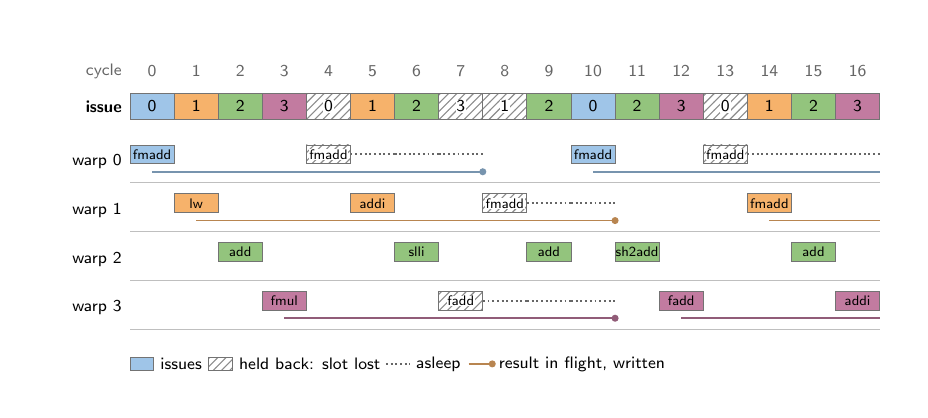
\begin{tikzpicture}[x=1cm, y=1cm,
  tbl/.style={draw=black!55, line width=0.35pt},
  panel/.style={draw=none, fill=none},
  lbl/.style={font=\fs, inner sep=0.5pt},
  cell/.style={font=\fss, inner sep=0.3pt},
  note/.style={font=\fss, inner sep=0.5pt, align=left},
  subcap/.style={font=\fs, inner sep=1pt},
  held/.style={draw=black!55, pattern=north east lines, pattern color=black!45, line width=0.35pt},
  sleep/.style={draw=black!60, densely dotted, line width=0.7pt},
  arr/.style={-{Latex[length=1.3mm, width=0.9mm]}, line width=0.5pt}]

\draw[panel] (-0.100,-0.050) rectangle (10.970,4.550);
\node[cell, text=black!60] at (1.480,4.000) {0};
\node[cell, text=black!60] at (2.040,4.000) {1};
\node[cell, text=black!60] at (2.600,4.000) {2};
\node[cell, text=black!60] at (3.160,4.000) {3};
\node[cell, text=black!60] at (3.720,4.000) {4};
\node[cell, text=black!60] at (4.280,4.000) {5};
\node[cell, text=black!60] at (4.840,4.000) {6};
\node[cell, text=black!60] at (5.400,4.000) {7};
\node[cell, text=black!60] at (5.960,4.000) {8};
\node[cell, text=black!60] at (6.520,4.000) {9};
\node[cell, text=black!60] at (7.080,4.000) {10};
\node[cell, text=black!60] at (7.640,4.000) {11};
\node[cell, text=black!60] at (8.200,4.000) {12};
\node[cell, text=black!60] at (8.760,4.000) {13};
\node[cell, text=black!60] at (9.320,4.000) {14};
\node[cell, text=black!60] at (9.880,4.000) {15};
\node[cell, text=black!60] at (10.440,4.000) {16};
\node[note, anchor=east, text=black!60] at (1.120,4.000) {cycle};
\node[lbl, anchor=east] at (1.120,3.550) {\textbf{issue}};
\draw[tbl, fill=wA] (1.200,3.380) rectangle (1.760,3.720);
\node[cell] at (1.480,3.550) {0};
\draw[tbl, fill=wB] (1.760,3.380) rectangle (2.320,3.720);
\node[cell] at (2.040,3.550) {1};
\draw[tbl, fill=wC] (2.320,3.380) rectangle (2.880,3.720);
\node[cell] at (2.600,3.550) {2};
\draw[tbl, fill=wD] (2.880,3.380) rectangle (3.440,3.720);
\node[cell] at (3.160,3.550) {3};
\draw[held] (3.440,3.380) rectangle (4.000,3.720);
\node[cell, fill=white, inner sep=0.3pt] at (3.720,3.550) {0};
\draw[tbl, fill=wB] (4.000,3.380) rectangle (4.560,3.720);
\node[cell] at (4.280,3.550) {1};
\draw[tbl, fill=wC] (4.560,3.380) rectangle (5.120,3.720);
\node[cell] at (4.840,3.550) {2};
\draw[held] (5.120,3.380) rectangle (5.680,3.720);
\node[cell, fill=white, inner sep=0.3pt] at (5.400,3.550) {3};
\draw[held] (5.680,3.380) rectangle (6.240,3.720);
\node[cell, fill=white, inner sep=0.3pt] at (5.960,3.550) {1};
\draw[tbl, fill=wC] (6.240,3.380) rectangle (6.800,3.720);
\node[cell] at (6.520,3.550) {2};
\draw[tbl, fill=wA] (6.800,3.380) rectangle (7.360,3.720);
\node[cell] at (7.080,3.550) {0};
\draw[tbl, fill=wC] (7.360,3.380) rectangle (7.920,3.720);
\node[cell] at (7.640,3.550) {2};
\draw[tbl, fill=wD] (7.920,3.380) rectangle (8.480,3.720);
\node[cell] at (8.200,3.550) {3};
\draw[held] (8.480,3.380) rectangle (9.040,3.720);
\node[cell, fill=white, inner sep=0.3pt] at (8.760,3.550) {0};
\draw[tbl, fill=wB] (9.040,3.380) rectangle (9.600,3.720);
\node[cell] at (9.320,3.550) {1};
\draw[tbl, fill=wC] (9.600,3.380) rectangle (10.160,3.720);
\node[cell] at (9.880,3.550) {2};
\draw[tbl, fill=wD] (10.160,3.380) rectangle (10.720,3.720);
\node[cell] at (10.440,3.550) {3};
\node[lbl, anchor=east] at (1.120,2.850) {warp 0};
\draw[black!25, line width=0.3pt] (1.200,2.580) -- (10.720,2.580);
\draw[tbl, fill=wA] (1.200,2.820) rectangle (1.760,3.060);
\node[cell] at (1.480,2.940) {\fontsize{4.9}{5.4}\selectfont fmadd};
\draw[held] (3.440,2.820) rectangle (4.000,3.060);
\node[cell, fill=white, inner sep=0.2pt] at (3.720,2.940) {\fontsize{4.9}{5.4}\selectfont fmadd};
\draw[sleep] (4.000,2.940) -- (4.560,2.940);
\draw[sleep] (4.560,2.940) -- (5.120,2.940);
\draw[sleep] (5.120,2.940) -- (5.680,2.940);
\draw[tbl, fill=wA] (6.800,2.820) rectangle (7.360,3.060);
\node[cell] at (7.080,2.940) {\fontsize{4.9}{5.4}\selectfont fmadd};
\draw[held] (8.480,2.820) rectangle (9.040,3.060);
\node[cell, fill=white, inner sep=0.2pt] at (8.760,2.940) {\fontsize{4.9}{5.4}\selectfont fmadd};
\draw[sleep] (9.040,2.940) -- (9.600,2.940);
\draw[sleep] (9.600,2.940) -- (10.160,2.940);
\draw[sleep] (10.160,2.940) -- (10.720,2.940);
\draw[line width=0.6pt, draw=wA!75!black] (1.480,2.720) -- (5.680,2.720);
\fill[wA!75!black] (5.680,2.720) circle (0.045);
\draw[line width=0.6pt, draw=wA!75!black] (7.080,2.720) -- (10.720,2.720);
\node[lbl, anchor=east] at (1.120,2.230) {warp 1};
\draw[black!25, line width=0.3pt] (1.200,1.960) -- (10.720,1.960);
\draw[tbl, fill=wB] (1.760,2.200) rectangle (2.320,2.440);
\node[cell] at (2.040,2.320) {\fontsize{4.9}{5.4}\selectfont lw};
\draw[tbl, fill=wB] (4.000,2.200) rectangle (4.560,2.440);
\node[cell] at (4.280,2.320) {\fontsize{4.9}{5.4}\selectfont addi};
\draw[held] (5.680,2.200) rectangle (6.240,2.440);
\node[cell, fill=white, inner sep=0.2pt] at (5.960,2.320) {\fontsize{4.9}{5.4}\selectfont fmadd};
\draw[sleep] (6.240,2.320) -- (6.800,2.320);
\draw[sleep] (6.800,2.320) -- (7.360,2.320);
\draw[tbl, fill=wB] (9.040,2.200) rectangle (9.600,2.440);
\node[cell] at (9.320,2.320) {\fontsize{4.9}{5.4}\selectfont fmadd};
\draw[line width=0.6pt, draw=wB!75!black] (2.040,2.100) -- (7.360,2.100);
\fill[wB!75!black] (7.360,2.100) circle (0.045);
\draw[line width=0.6pt, draw=wB!75!black] (9.320,2.100) -- (10.720,2.100);
\node[lbl, anchor=east] at (1.120,1.610) {warp 2};
\draw[black!25, line width=0.3pt] (1.200,1.340) -- (10.720,1.340);
\draw[tbl, fill=wC] (2.320,1.580) rectangle (2.880,1.820);
\node[cell] at (2.600,1.700) {\fontsize{4.9}{5.4}\selectfont add};
\draw[tbl, fill=wC] (4.560,1.580) rectangle (5.120,1.820);
\node[cell] at (4.840,1.700) {\fontsize{4.9}{5.4}\selectfont slli};
\draw[tbl, fill=wC] (6.240,1.580) rectangle (6.800,1.820);
\node[cell] at (6.520,1.700) {\fontsize{4.9}{5.4}\selectfont add};
\draw[tbl, fill=wC] (7.360,1.580) rectangle (7.920,1.820);
\node[cell] at (7.640,1.700) {\fontsize{4.9}{5.4}\selectfont sh2add};
\draw[tbl, fill=wC] (9.600,1.580) rectangle (10.160,1.820);
\node[cell] at (9.880,1.700) {\fontsize{4.9}{5.4}\selectfont add};
\node[lbl, anchor=east] at (1.120,0.990) {warp 3};
\draw[black!25, line width=0.3pt] (1.200,0.720) -- (10.720,0.720);
\draw[tbl, fill=wD] (2.880,0.960) rectangle (3.440,1.200);
\node[cell] at (3.160,1.080) {\fontsize{4.9}{5.4}\selectfont fmul};
\draw[held] (5.120,0.960) rectangle (5.680,1.200);
\node[cell, fill=white, inner sep=0.2pt] at (5.400,1.080) {\fontsize{4.9}{5.4}\selectfont fadd};
\draw[sleep] (5.680,1.080) -- (6.240,1.080);
\draw[sleep] (6.240,1.080) -- (6.800,1.080);
\draw[sleep] (6.800,1.080) -- (7.360,1.080);
\draw[tbl, fill=wD] (7.920,0.960) rectangle (8.480,1.200);
\node[cell] at (8.200,1.080) {\fontsize{4.9}{5.4}\selectfont fadd};
\draw[tbl, fill=wD] (10.160,0.960) rectangle (10.720,1.200);
\node[cell] at (10.440,1.080) {\fontsize{4.9}{5.4}\selectfont addi};
\draw[line width=0.6pt, draw=wD!75!black] (3.160,0.860) -- (7.360,0.860);
\fill[wD!75!black] (7.360,0.860) circle (0.045);
\draw[line width=0.6pt, draw=wD!75!black] (8.200,0.860) -- (10.720,0.860);
\draw[tbl, fill=wA] (1.200,0.200) rectangle (1.500,0.360);
\node[note, anchor=west] at (1.560,0.280) {issues};
\draw[held] (2.200,0.200) rectangle (2.500,0.360);
\node[note, anchor=west] at (2.560,0.280) {held back: slot lost};
\draw[sleep] (4.450,0.280) -- (4.750,0.280);
\node[note, anchor=west] at (4.810,0.280) {asleep};
\draw[line width=0.6pt, draw=wB!75!black] (5.500,0.280) -- (5.800,0.280);
\fill[wB!75!black] (5.800,0.280) circle (0.045);
\node[note, anchor=west] at (5.860,0.280) {result in flight, written};
\end{tikzpicture}
\end{document}
